\documentclass[12pt]{article}
\usepackage{tikz}
\usepackage{circuitikz}
\usepackage{amsmath}
\usepackage{amssymb}
\usepackage{graphicx}
\usepackage{float}
\usepackage{geometry}
\usepackage{pgfplots}
\usepackage{color}
\usepackage{xcolor}

\geometry{a4paper, margin=1in}
\pgfplotsset{compat=1.18}

\begin{document}

Analyze the network topology:

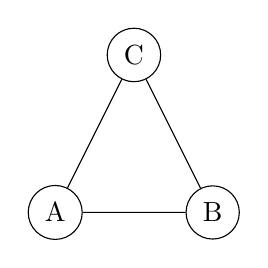
\begin{tikzpicture}
\draw (0,0) node[circle,draw] (A) {A};
\draw (2,0) node[circle,draw] (B) {B};
\draw (1,2) node[circle,draw] (C) {C};
\draw (A) -- (B) -- (C) -- (A);
\end{tikzpicture}

a) Identify the topology type
b) How many connections are needed for n nodes?
c) What happens if one connection fails?

\end{document}
